\documentclass{resume}
\usepackage{zh_CN-Adobefonts_external, tabu, multirow, linespacing_fix, cite, titlesec, graphicx, amsmath, fontawesome5,eso-pic}

% Adjust section and subsection spacing
\titlespacing*{\section}{0pt}{0.5ex plus 0.2ex minus 0.2ex}{0.5ex plus 0.2ex}
\titlespacing*{\subsection}{0pt}{0.5ex plus 0.2ex minus 0.2ex}{0.5ex plus 0.2ex}

% Set paragraph and item spacing
\setlength{\parskip}{0.5ex}
\setlength{\itemsep}{0.5ex}

% Add profile photo background
\AddToShipoutPictureBG*{%
  \AtPageLowerLeft{%
    \put(456,701){%
      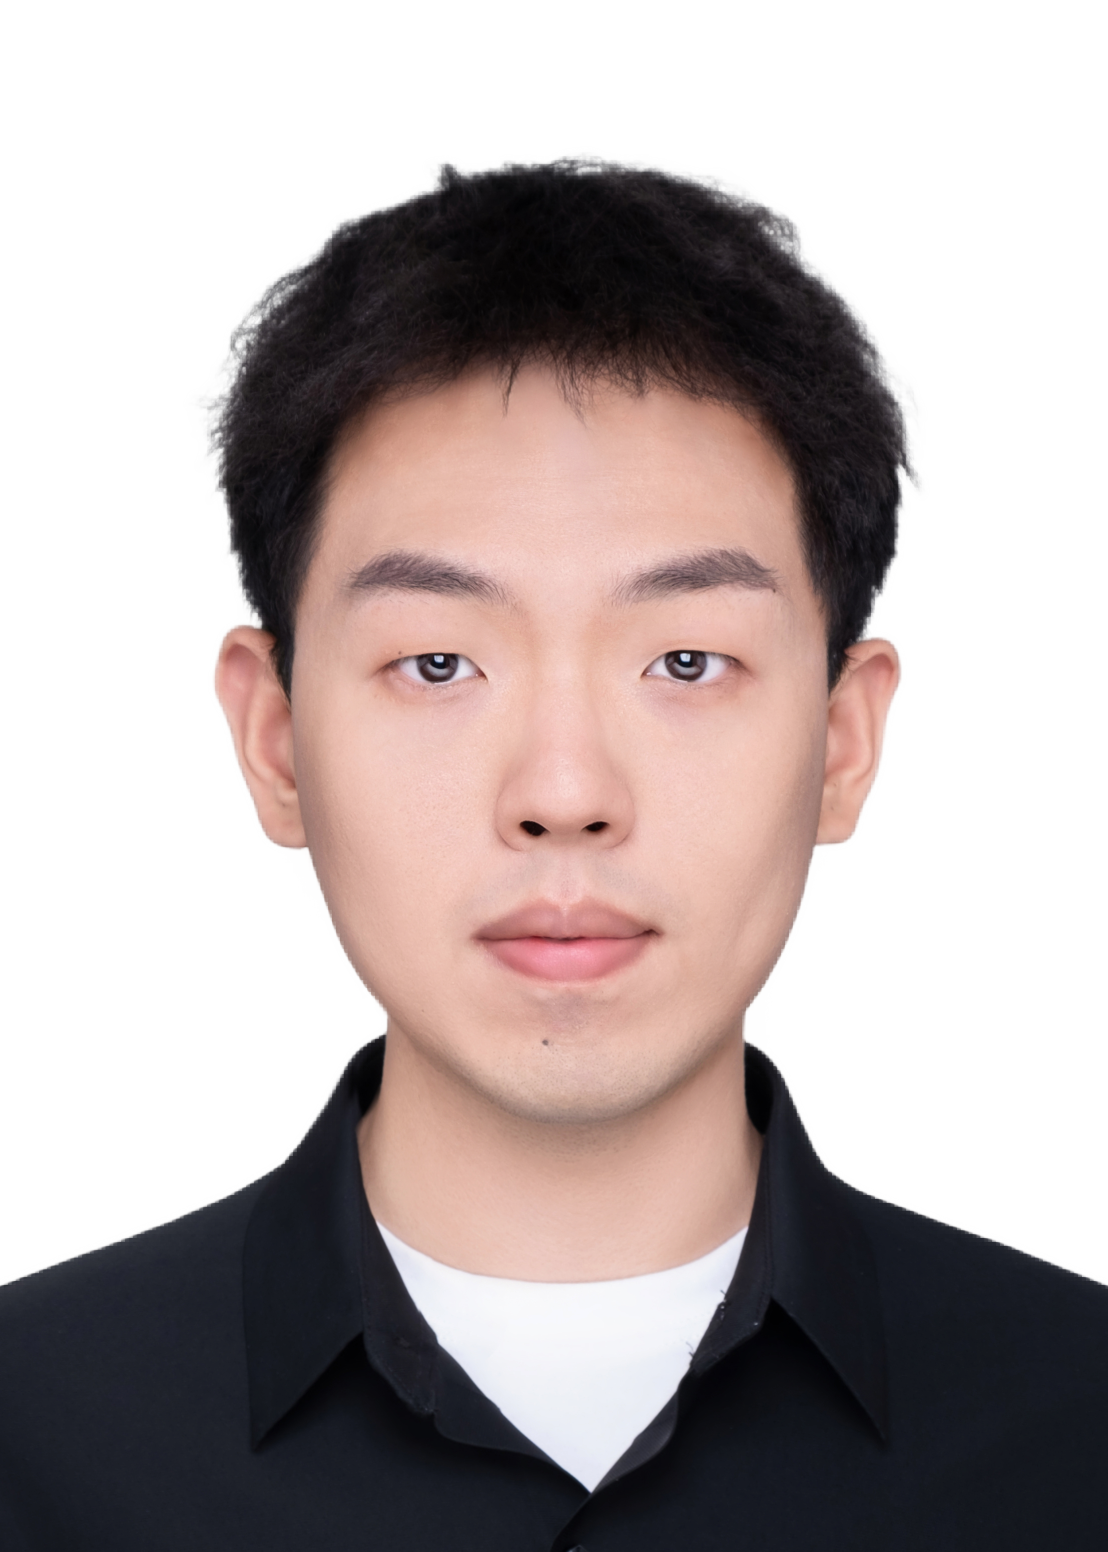
\includegraphics[width=1.15in]{avatar}
    }%
  }%
}

\begin{document}
\pagestyle{empty}

\name{Yinqiao Li}
\basicInfo{
    \email{865562832@qq.com} \textperiodcentered\ 
    \phone{152-2510-8555} \textperiodcentered\ 
    \text{Born in April 2001}
  }
\basicInfo{Strong English proficiency, computer operation and interpersonal communication skills}

\section{\faGraduationCap\ Education}
\datedsubsection{\textbf{Central China Normal University, University of Wollongong (QS162)}}{September 2023 -- June 2025}
\textbf{Dual Master's Degree in Computer Technology and Computer Science} \\
Core Courses: Python Data Structures, Project Management, SQL, Machine Learning, Cryptography, Data Mining, Advanced Network Security \\
Awarded \textbf{Full Scholarship for 2024-2025 Academic Year (80,000 RMB)}, IELTS 6.5 \textbf{(Reading 8, Listening 7)} \\
Served as Graduate Party Branch Secretary, managing daily party affairs, recognized as Outstanding Graduate Student Leader

\datedsubsection{\textbf{Zhengzhou University of Aeronautics}}{September 2019 -- June 2023}
Bachelor of Engineering in Materials Science and Engineering (Functional Materials) with GPA 3.44, Minor in English \\
\textbf{University-level Outstanding Student, Second-class Scholarship, Second Prize in National College English Competition}

\section{\faUsers\ Work Experience}
\datedsubsection{\textbf{Shanghai Pansong Private Equity Fund Management Co., Ltd. - Operations Engineer}}{June 2024 -- September 2024}
\begin{itemize}
  \item Object Storage Work: Implemented disaster recovery for production environment code, logs, and databases using public cloud services; completed preliminary research, pricing analysis, procurement coordination, deployment, and parameter optimization
  \item Python Operations Code Optimization: Developed command-line interface using Python's argparse module to selectively rerun specific functions after program crashes
  \item Server Capacity Expansion: Troubleshot MongoDB slow query issues, identified low cache hit rate, implemented Linux server memory expansion; Performed RAID 5 expansion on Windows servers for MySQL master-slave synchronization SSD space requirements
  \item Data Provider Deployment: Converted Docker-Compose deployment to Kubernetes Deployment using Dockerfile; Completed test environment deployment for three data providers and one intraday (T+0) trading software
\end{itemize}

\section{\faUsers\ Project Experience}
\datedsubsection{\textbf{Driver Fatigue Monitoring Method Based on Multimodal and rPPG Technology}}{September 2023 -- June 2025}
Computer Vision, Deep Learning, Python, Two National Natural Science Foundation Projects Initiated, One Completed
\begin{itemize}
  \item Extracted rPPG physiological signals from visual data to obtain heart rate, heart rate variability, and respiratory data
  \item Implemented feature extraction and processing of multimodal features using CNN, with LSTM for temporal feature sharing
  \item Achieved feature-level and decision-level fusion for multimodal feature processing
  \item Developed 3DCNN + temporal normalization + SimAM attention mechanism, achieving comparable performance to PhysNet model with half the parameters
\end{itemize}

\datedsubsection{\textbf{Airport Runway Debris Removal Robot}}{April 2020 -- September 2021}
Intelligent cleaning robot for airport runways based on path planning algorithms and computer vision, built using OpenCV library and Raspberry Pi
\begin{itemize}
  \item Led team from project inception to completion, coordinated work progress, frequently served as presenter with extensive on-site experience
  \item Obtained patent "An Airport Runway Debris Removal Device" (Patent No.: 202120932618.7)
  \item Won First Prize in Zhengzhou Aeronautics Institute Challenge Cup, Second Prize in Henan Province Challenge Cup, and Second Prize in Henan Province Internet+ Competition as a first-year project
\end{itemize}

\section{\faHeartO\ Research Experience}
\datedsubsection{\textbf{Automatic Knowledge Graph Construction over Efficient Information Extraction Networks, IEIR 2023 Conference}}{July 2023 -- November 2023}
\begin{itemize}
  \item Project Background: Aimed to reduce pre-training model costs and improve runtime speed while maintaining named entity recognition accuracy for building knowledge graphs from small sample datasets
  \item Solution: Implemented CNN+Bi-LSTM+Attention mechanism, achieving comparable F1-score of 0.8243 to RoBERTa+CRF model while reducing runtime by 50\%
\end{itemize}

\end{document}